 \documentclass[11pt]{article}

  \usepackage{smoothing_paper}
\usepackage[section]{placeins}
\usepackage{tabularx,ragged2e,booktabs,caption}

\interfootnotelinepenalty=10000

%%%%%%%%%%%%%%%%%%%%%%%%%%%%%%%%chiheb commands

\newcommand{\ie}{\emph{i.e.}}
\newcommand{\eg}{\emph{e.g.}}
\newcommand{\cf}{\emph{cf.}}
\newcommand{\prob}[1]{\mathrm{P}\left(#1\right)}
\newcommand{\expt}[1]{\mathrm{E}\left[#1\right]}
\newcommand{\expth}[1]{\hat{\mathrm{E}}\left[#1\right]}



\newcommand{\rset}{\mathbb{R}}
\newcommand{\nset}{\mathbb{N}}
\newcommand{\zset}{\mathbb{Z}}



\newcommand{\PERIOD}{.}
\newcommand{\COMMA}{,}
\newcommand{\BIGSPACE}{\,\,\,\,\,\,\,}



\newcommand{\Ordo}[1]{{\mathcal{O}}\left(#1\right)}
\newcommand{\ordo}[1]{{o}\left(#1\right)}

%%%%%%%%%%%%%%%%%%%%%%%%%%%%%%%%%%%%%%%%%%%%%%%%%%%%%%%%%%%%%%%%%%%%%%%%
%%
%% DO WE RELLY NEED THE FOLLOWING??

%%  new margin
%%%%%%%%%%%%%%%%%%%%%%%%%%%%%%%%%%%%%%%%%%%
\pagestyle{plain}                                                      %%
%%%%%%%%%% EXACT 1in MARGINS %%%%%%%                                   %%
\setlength{\textwidth}{6.5in}     %%                                   %%
\setlength{\oddsidemargin}{0in}   %%   
\setlength{\evensidemargin}{0in}  %%        
\setlength{\textheight}{8.5in}    %%       
\setlength{\topmargin}{-0.2in}    %%   
\setlength{\headheight}{0in}      %%    
\setlength{\headsep}{0in}         %%                   
\setlength{\footskip}{.5in}       %%                       
%%%%%%%%%%%%%%%%%%%%%%%%%%%%%%%%%%%%                                   %%
\newcommand{\required}[1]{\section*{\hfil #1\hfil}}                    %%
\renewcommand{\refname}{\hfil References Cited\hfil}                   %%

\def\SMALLSKIP{\smallskip}
\def\MEDSKIP{\medskip}
\def\BIGSKIP{\bigskip}

%%
%%%%%%%%%%%%%%%%%%%%%%%%%%%%%%%%%%%%%%%%%%%%%%%%%%%%%%%%%%%%%%%%%%%%%

\makeatletter
\def\BState{\State\hskip-\ALG@thistlm}
\makeatother



%%%%%%%%%%%%%%%%%%%%%%%%%%%%%%%%%%%%%%%%

\title{On the choice of the numerical scheme for the simulation of the Heston model} 
    \date{ }

\begin{document}
\maketitle






\section{Options under the discretized the Heston model}
In this section, we consider  testing options under the discretized Heston model \cite{heston1993closed,broadie2006exact,kahl2006fast,andersen2007efficient} whose dynamics are given by
\begin{align}\label{eq:dynamics Heston}
dS_t&=\mu S_t dt+\sqrt{v_t}S_t dW_t^S= \mu S_t dt+ \rho\sqrt{v_t}S_t dW_t^v+ \sqrt{1-\rho^2} \sqrt{v_t}S_t dW_t \nonumber\\
dv_t&=\kappa (\theta-v_t)dt+\xi \sqrt{v_t} dW_t^v\COMMA
\end{align}
where 

\begin{itemize}
\item $S_t$ is the price of the asset, $v_t$ the instantaneous variance, given as  a CIR process.
\item $W_{t}^{S},W_{t}^{v}$ are correlated Wiener processes with correlation $\rho$.
\item $\mu$  is the rate of return of the asset.
\item $\theta$ is  the mean  variance.
\item $\kappa$ is the rate at which $v_t$ reverts to $\theta$.
\item $\xi$ is the volatility of the volatility, and determines the variance of $v_t$.
\end{itemize}
\subsection{Schemes to simulate the Heston dynamics}\label{sec:Schemes to simulate the Heston dynamics}
Given that the SDE for the asset path is now dependent  upon the solution of the second volatility SDE in \eqref{eq:dynamics Heston}, it is necessary to simulate the volatility process first and then utilize this "volatility path" in order to simulate the asset path. In the case of the original GBM SDE it is possible to use It\^o's Lemma to directly solve for $S_t$. However, we are unable to utilize that procedure here and must use a numerical approximation in order to obtain both paths. In the following, we try to give an overview of the methods that we can use in our context. These methods mainly differs by the way it simulates the volatility process to ensure its positiveness.
\subsubsection{Fixed Euler scheme}\label{sec:Discretization of Heston model with a non smooth transformations for the volatility process}
In this context, one can use Forward Euler scheme to simulate the Heston model, and to avoid  problems with negative values of the volatility process $v_t$, many fixes  were introduced in the literature (see \cite{lord2010comparison}). We introduce $f_1, f_2$, and $f_3$, which with different choices implies different schemes, and   apply Forward Euler scheme to discretize \ref{eq:dynamics Heston}  results in
\begin{align}\label{eq:FE_Heston_discrete}
\hat{S}_{t+\Delta t}&= \hat{S}_t +\mu \hat{S}_t \Delta t+\sqrt{\hat{V}_t \Delta t} \hat{S}_t Z_s \nonumber\\
\hat{V}_{t+\Delta t}&=f_1(\hat{V}_t)+\kappa (\theta-f_2(\hat{V}_t)) \Delta t+\xi \sqrt{f_3(\hat{V}_t) \Delta t} Z_V \nonumber\\
\hat{V}_{t+\Delta t}&=f_3(\hat{V}_{t+\Delta t}) \COMMA
\end{align}
where $Z_s$ and $Z_V$  are two correlated standard normal variables with correlation $\rho$, such that $Z_s=\rho Z_V+\sqrt{1-\rho^2} Z_t$. 

\FloatBarrier
\begin{table}[h!]
	\centering
	\begin{tabular}{l*{6}{c}r}
		\toprule[1.5pt]
	Scheme &  $f_1$& $f_2$  & $f_3$     \\
	\hline
	full truncation scheme & $\hat{V}_t$ &  $\hat{V}_t^+$&$\hat{V}_t^+$\\
	Partial truncation scheme & $\hat{V}_t$ &  $\hat{V}_t$&$\hat{V}_t^+$\\
	The reflection scheme  &$\abs{\hat{V}_t}$ & $\abs{\hat{V}_t}$& $\abs{\hat{V}_t}$\\
			\bottomrule[1.25pt]
	\end{tabular}
	\label{Numerical schemes for CIR process}
\end{table}
\FloatBarrier
where  $\hat{V}_t^+=\max(0,\hat{V}_t)$.

\cite{lord2010comparison} suggest that the Full Truncation method is the optimal option in terms of weak error convergence and robustness with respect to the parameters of the model. Therefore,  we use this scheme for this approach. 

\subsection{Euler schemes with moment matching}\label{sec:Euler schemes with moment matching}
We consider two moment matching Euler schemes that were suggested by Andersen and Brotherton-Ratcliffe \cite{andersen2005extended} (we call it ABR scheme) and by Anderson in \cite{andersen2007efficient} (we choose the QE method that was reported to have the optimal results). 
\subsubsection{The ABR method}\label{sec:The ABR method}
The ABR method is suggested in \cite{andersen2005extended}, where the
variance $v$ is assumed to be locally lognormal, where the parameters are determined such that the first two moments of the discretization coincide with the theoretical moments, that is 
\begin{align}\label{eq: vol_moment_matching}
\hat{V}(t+\Delta t)&= \left(e^{-\kappa \Delta t}  \hat{V}(t) + \left( 1-e^{-\kappa \Delta t}\right) \theta  \right) e^{-\frac{1}{2} \Gamma(t)^2 \Delta t+\Gamma(t) \Delta W_v(t)}\nonumber\\
\Gamma(t)^2 &=\Delta t^{-1} \log \left(  1+ \frac{\frac{1}{2}\xi^2 \kappa^{-1} \hat{V}(t) (1-e^{-2 \kappa \Delta t})}{\left( e^{-\kappa \Delta t} \hat{V}(t) +(1-e^{- \kappa \Delta t}) \theta \right)^2 }\right)
\end{align}
As reported in \cite{lord2010comparison}, the scheme, being very easy to implement, is much more effective than many of the Euler fixes, however, it was reported that it has a bad weak error behavior that is not robust with parameters values, which is something that we need to check in our setting!
\subsubsection{The QE method}\label{sec:The QE method}
On the other hand, and using the same idea of moment matching, Anderson in\cite{andersen2007efficient}, suggested  more discretisations for the Heston model similar to \eqref{eq: vol_moment_matching} and taking the shape of the Heston density function into
account.  These schemes have negligible bias, at the cost of a more complex implementation than  the one introduced by \cite{andersen2005extended}. As reported by \cite{andersen2007efficient}, the QE method is the optimal scheme to use and it follows the following algorithm.
\begin{enumerate}
\item Select some arbitrary level $\Psi_c \in [1,2]$.
\item  Given $\hat{V}(t)$, compute $m$ and $s^2$ given by
\begin{align*}
m &=\expt{V(t+\Delta t) \mid V(t)=\hat{V}(t)}=\theta+(\hat{v}(t)-\theta) e^{-\kappa \Delta t} \\
s^2 &= \text{Var}\left[V(t+\Delta t) \mid V(t)=\hat{V}(t)\right]=\frac{\hat{V}(t) \xi^2 e^{-\kappa \Delta t}}{\kappa} (1-e^{-\kappa \Delta t}) +\frac{\theta \xi^2}{2 \kappa} (1-e^{-\kappa \Delta t})^2.
\end{align*}
\item Compute $\Psi=s^2/m^2$.
\item Draw a uniform random number $U_V$.
\item If $\Psi\le \Psi_c$
\begin{enumerate}
\item[i)] Compute $a$ and $b$ given by
\begin{align*}
b^2&=2 \Psi^{-1}-1+\sqrt{2 \Psi^{-1}}\sqrt{2 \Psi^{-1}-1}\\
a&=\frac{m}{1+b^2}
\end{align*}
\item[ii)] Compute $Z_V=\Phi^{-1}(U_V)$, where $\Phi^{-1}$ is the inverse cumulative
Gaussian distribution function.
\item[iii)] Set $\hat{V}(t+\Delta t)=a(b+Z_V^2)^2$.
\end{enumerate}
\item Otherwise, if $\Psi >\Psi_c$

\begin{enumerate}
\item[i)] Compute $p$ and $\beta$ according to 
\begin{align*}
p&=\frac{\Psi-1}{\Psi-1}\\
\beta&=\frac{1-p}{m}
\end{align*}
\item[ii)] Set $\hat{V}(t+\Delta t)=h^{-1}(U_V; p,\beta)$, where $h^{-1}$ is given by

 \[
    h^{-1}(u; p,\beta)=\left\{
                \begin{array}{ll}
                  0, \quad  0 \le u \le p\\
                   \beta^{-1} \log\left(\frac{1-p}{1-u}\right), \quad  p< u \le 1
                \end{array}
              \right.
  \]
\end{enumerate}
\end{enumerate}

Compared to ABR scheme, the QE scheme may have a better weak error behavior with the disadvantage of being more costly. Furthermore, the QE algorithm uses two different distributions to model the volatility depending on the initial value of the volatility!
\subsection{Kahl-Jackel Scheme}
\cite{kahl2006fast} suggested discretizing the volatility process using an implicit Milstein scheme, coupled with their “IJK” discretization for the stock process. Specifically, they propose the scheme
\begin{align}
\log(\hat{X}(t+\Delta t))&=\log(\hat{X}(t))-\frac{\Delta t}{4} \left(\hat{V}(t+\Delta t)+ \hat{V}(t) \right) +\rho \sqrt{\hat{V}(t)} Z_V \sqrt{\Delta t}  \nonumber\\
& +\frac{1}{2} \left(\sqrt{\hat{V}(t+\Delta t)}+ \sqrt{\hat{V}(t)} \right) \left(Z_x \sqrt{\Delta t}- \rho Z_V \sqrt{\Delta t}  \right) +\frac{\xi}{2} \rho  \Delta t (Z_V^2-1) \nonumber\\
 \hat{V}(t+\Delta t)&=\frac{\hat{V}(t)+\theta \kappa \Delta t+\xi \sqrt{\hat{V}(t)} Z_V \sqrt{\Delta t} +\frac{\xi^2}{4} \Delta t (Z_V^2-1) }{1+ \kappa \Delta t }
\end{align}

It is easy to check that this discretization scheme will result in positive paths for the $V$ process if $4 \kappa \theta >\xi^2$ (which is rarely satisfied in practice). Unfortunately \cite{kahl2006fast} does not provide a solution for this problem, but it seems reasonable to use a truncation scheme similar to those presented in Section \ref{sec:Discretization of Heston model with a non smooth transformations for the volatility process}.  Therefore, we do not test this scheme in our numerical experiments since we think that it will have similar issues that we observed for the full truncation scheme presented in Section \ref{sec:Discretization of Heston model with a non smooth transformations for the volatility process}. Furthermore, it was shown that the convergence of the weak rate of the IJK-IMM scheme  somewhat erratic, especially for cases  $4 \kappa \theta \le \xi^2$.

\subsection{Discretization of Heston model with the volatility process Simulated using the sum of  Ornstein-Uhlenbeck (Bessel) processes}\label{sec:Discretization of Heston model with the volatility process Simulated using the sum of  Ornstein-Uhlenbeck (Bessel) processes}

Since we are using ASGQ which is very sensitive to the smoothness of the integrand. We found numerically (see section \ref{sec:On the choice of the simulation scheme of the Heston model}) that using a non smooth transformation to ensure the positiveness of the volatility process deteriorates the performance of the ASGQ. An alternative way to guarantee the positiveness of the volatility process is to simulate it as  the sum of  Ornstein-Uhlenbeck (Bessel) processes.

In fact, it is well known that any Ornstein-Uhlenbeck (OU) process is normally distributed. Thus, the sum of $n$ squared OU processes is chi-squared distributed with $n$ degrees of freedom, where $n \in \nset$. Let us define $\mathbf{X}$ to be a $n$-dimensional vector valued OU process with
\begin{equation}\label{equivalent OU process} 
\mathrm{d}X_t^i = \alpha X_t^i \mathrm{d}t + \beta \mathrm{d}W_t^i,
\end{equation}
where $\mathbf{W}$ is a $n$-dimensional vector of independent Brownian motions. 

We define also the process $Y_t$ as  
\begin{equation}
Y_t = \sum_{i = 1}^n \left( X_t^i \right)^2.
\end{equation}
Then, using the fact that
\begin{eqnarray}
\mathrm{d} \left( X_t^i \right)^2 & = & 2 X_t^i \mathrm{d}X_t^i + 2 \mathrm{d} \langle X^i \rangle_t \nonumber\\
& = & \left( 2 \alpha \left( X_t^i \right)^2 + \beta^2 \right) \mathrm{d}t + 2 \beta X_t^i \mathrm{d}W_t^i,
\end{eqnarray}
we can write
\begin{eqnarray}\label{eq:expressing CIR processes from OU processes}
\mathrm{d}Y_t & = & \mathrm{d} \left( \sum_{i = 1}^n \left( X_t^i \right)^2 \right) \nonumber\\
& = & \sum_{i = 1}^n \mathrm{d} \left( X_t^i \right)^2 \nonumber\\
& = & \left( 2 \alpha Y_t + n \beta^2 \right) \mathrm{d}t + 2 \beta \sum_{i = 1}^n X_t^i \mathrm{d}W_t^i,
\end{eqnarray}
where the second step follows from the independence of the Brownian motions. Furthermore, we  note that the process
\begin{equation}
Z_t = \int_0^t \sum_{i = 1}^n X_u^i \mathrm{d}W_u^i
\end{equation}
is a martingale with quadratic variation
\begin{eqnarray}
\langle Z \rangle_t & = & \int_0^t \sum_{i = 1}^n \left( X_u^i \right)^2 \mathrm{d}u \nonumber\\
& = & \int_0^t Y_u \mathrm{d}u.
\end{eqnarray}
Consequently, by L\'evy's characterization theorem, we can show that the process
\begin{equation}
\widetilde{W}_t = \int_0^t \frac{1}{\sqrt{Y_u}} \sum_{i = 1}^n X_u^i \mathrm{d}W_u^i
\end{equation}
is a Brownian motion.

Finally, we have 
\begin{eqnarray}\label{eq:equivalent CIR process}
\mathrm{d}Y_t & = & \left( 2 \alpha Y_t + n \beta^2 \right) \mathrm{d}t + 2 \beta \sqrt{Y_t} \mathrm{d}\tilde{W}_t \nonumber\\
& = & \kappa \left( \theta - Y_t \right) \mathrm{d}t + \xi \sqrt{Y_t} \mathrm{d}W_t,
\end{eqnarray}
where $\kappa = -2 \alpha$, $\theta = -n \beta^2 / 2 \alpha$ and $\xi = 2 \beta$.

Equations \eqref{equivalent OU process}, \eqref{eq:expressing CIR processes from OU processes}, and \eqref{eq:equivalent CIR process} show  in order to simulate the process $Y_t$ given by \eqref{eq:equivalent CIR process}, we can  simulate the  OU process  $\mathbf{X}$, with dynamics given by \eqref{equivalent OU process} such that its parameters $(\alpha, \beta)$ are expressed in terms of  those of the  process $Y_t$, that is 
$$ \alpha=-\frac{\kappa}{2},\quad \beta=\frac{\xi}{2}, \quad n=\frac{-2 \theta \alpha}{\beta^2}=\frac{4 \theta  \kappa}{\xi^2}.$$ Therefore, we conclude that we can simulate the volatility of the Heston model using a sum of OU processes.

\begin{remark}
The previous derivation can can be generalized to cases where $n$ is not an integer by considering a time-change of a squared Bessel process (see Chapter 6 in \cite{jeanblanc2009mathematical} for details). 
\end{remark}

\subsection{On the choice of the simulation scheme of the Heston model}\label{sec:On the choice of the simulation scheme of the Heston model}
In this section, we try to determine the optimal  scheme for simulating the Heston model defined in \ref{eq:dynamics Heston}.  In the literature  \cite{andersen2007efficient, lord2010comparison,alfonsi2010high}, more focus was on designing schemes that i) ensures the positiveness  of the volatility process and ii) has a good weak error behavior. In our setting, an optimal scheme is defined through two properties: i) the behavior of mixed rates which is an important feature for an  optimal performance of ASGQ, and  ii) the behavior of the weak error in order to apply Richardson extrapolation when it is needed. 
\subsubsection{Comparison in terms of mixed differences rates}
In this section, we try to compare  the four  approaches, discussed  in Section \ref{sec:Schemes to simulate the Heston dynamics}, which are : i) the full truncation scheme discussed in Section \ref{sec:Discretization of Heston model with a non smooth transformations for the volatility process},  ii) the ABR scheme discussed in Section \ref{sec:The ABR method},  ii) the QE scheme discussed in Section \ref{sec:The QE method}, and iv) the smooth scheme bases on sum of square of OU processes discussed in Section \ref{sec:Discretization of Heston model with the volatility process Simulated using the sum of  Ornstein-Uhlenbeck (Bessel) processes}. The comparison is done in terms of mixed differences convergence (defined in \eqref{eq:Work_error_contributions}) rates  which, as pointed out in \cite{haji2016multi}, are a key determinant for the optimal performance of ASGQ.
\begin{align}\label{eq:Work_error_contributions}
\Delta E_{\boldsymbol{\beta}} &= \abs{Q^{\mathcal{I} \cup \{\boldsymbol{\beta}\}}_N-Q^{\mathcal{I}}_N}.
\end{align}
For comparison, we use basically four sets of examples  given in table \ref{table:Reference solution, for different parameter constellations.}. The first two sets of parameters we used we test two different cases where the first case corresponds to $n=1$ and the second one corresponds to $n=2$. On the other hand, for the two remaining sets we used similar parameters tested in \cite{lord2010comparison}, where the set $3$  stems from Broadie and Kaya \cite{broadie2006exact}, and is the hardest of all examples. The example of set $4$ parameters  stems from Andersen \cite{andersen2007efficient}, where it is used to represent the market for long-dated FX options.  We also point out that only the second set of parameters  satisfies the Feller condition, that is $4 \kappa \theta > \xi^2$.

\FloatBarrier
\begin{table}[!h]
	\centering
	\begin{small}
	\begin{tabular}{l*{2}{c}r}
	\toprule[1.5pt]
		Parameters            & Reference solution    \\
		\hline

			Set $1$:	 $S_0=K=100$, $v_0=0.04$, $\mu=0$,  $\rho=-0.9$, $\kappa=1$, $\xi=0.1$, $\theta=\frac{\xi^2}{4 \kappa}=0.0025$, $(n=1)$.  & $6.332542$  \\	
				Set $2$: $S_0=K=100$, $v_0=0.04$, $\mu=0$,  $\rho=-0.9$, $\kappa=1$, $\xi=0.1$, $\theta=\frac{\xi^2}{4 \kappa}=0.005$, $(n=2)$.  & $6.445535$  \\	
					Set $3$:	$S_0=K=100$, $v_0=0.09$, $\mu=0$,  $\rho=-0.3$, $\kappa=2.7778$, $\xi=1$, $\theta=\frac{\xi^2}{4 \kappa}=0.09$, $(n=1)$.  & $10.86117$   \\
						Set $4$:	$S_0=K=100$, $v_0=0.04$, $\mu=0$,  $\rho=-0.9$, $\kappa=0.5$, $\xi=1$, $\theta=0.04$.  & $4.403384$\\
	\bottomrule[1.25pt]
	\end{tabular}
\end{small}
	\caption{Reference solution using Premia with cf\_call\_heston method as explained in \cite{heston1993closed}, for different parameter constellations. By $n$ we refer to the number of OU processes for simulating the volatility process in approach given by Section \ref{sec:Discretization of Heston model with the volatility process Simulated using the sum of  Ornstein-Uhlenbeck (Bessel) processes}}
	\label{table:Reference solution, for different parameter constellations.}
\end{table}
\FloatBarrier

In our numerical experiments, we only observed differences of mixed differences rates related to volatility coordinates, which is expected since we use basically schemes that only differ by the way it simulates the volatility process. Figures \ref{fig:first_diff_Heston_call_N_4_set2}, \ref{fig:first_diff_Heston_call_N_4_set3}, \ref{fig:first_diff_Heston_call_N_4_set4} and \ref{fig:first_diff_Heston_call_N_4_set5} show a comparison of first differences rates related to volatility coordinates for the different schemes and for the different examples. From this Figures, we have the following conclusions
\begin{enumerate}
\item In all examples, the full truncation scheme is the worst scheme to use in terms of first differences rates.
\item The scheme based on the sum of square of OU processes have a good performance for the first two sets. However, surprisingly, we observed a very bad performance for the example of Set $3$ parameters! 
\item  Both schemes based on moment matching (ABR and QE schemes) have the best performance in terms of mixed rates convergence and also they show robust behavior with respect to all examples with almost similar performance
\end{enumerate}
 
 \subsubsection*{Mixed differences for the case of Set 1 parameters}
\FloatBarrier
\begin{figure}[htb]
	\centering % <-- added
	\begin{subfigure}{0.4\textwidth}
		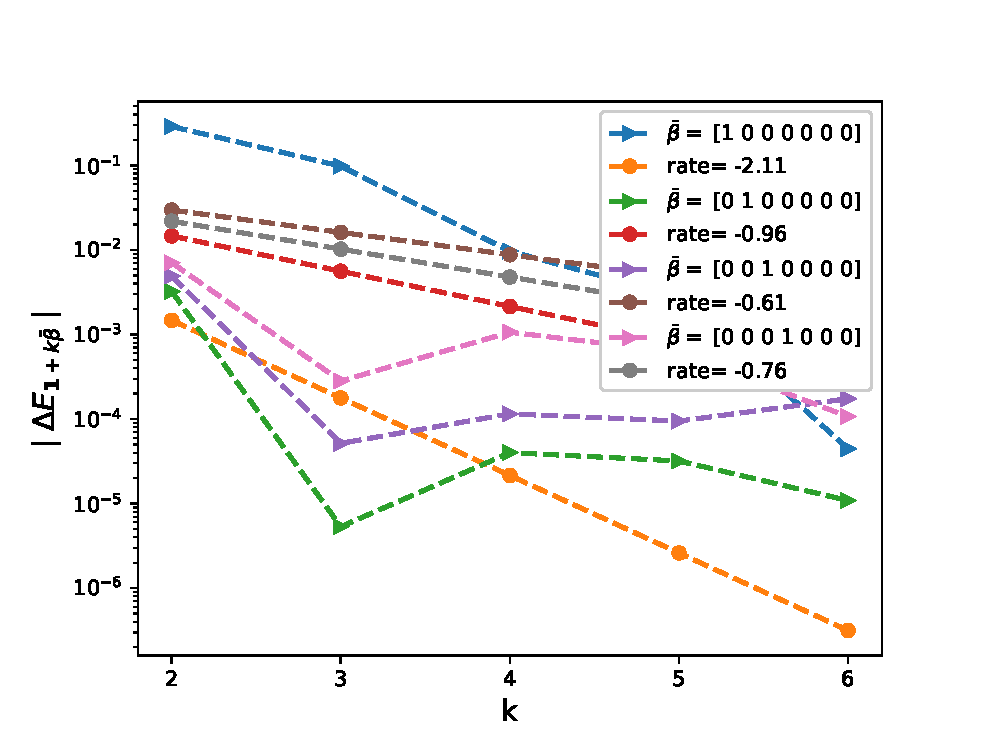
\includegraphics[width=\linewidth]{./figures/Heston_single_call_full_truncation_vol/mixed_rates/set2/N_4/first_difference_heston_4steps_hierarchical_2}
		\caption{}
		\label{fig:1}
	\end{subfigure}\hfil %% <-- added
	\begin{subfigure}{0.4\textwidth}
		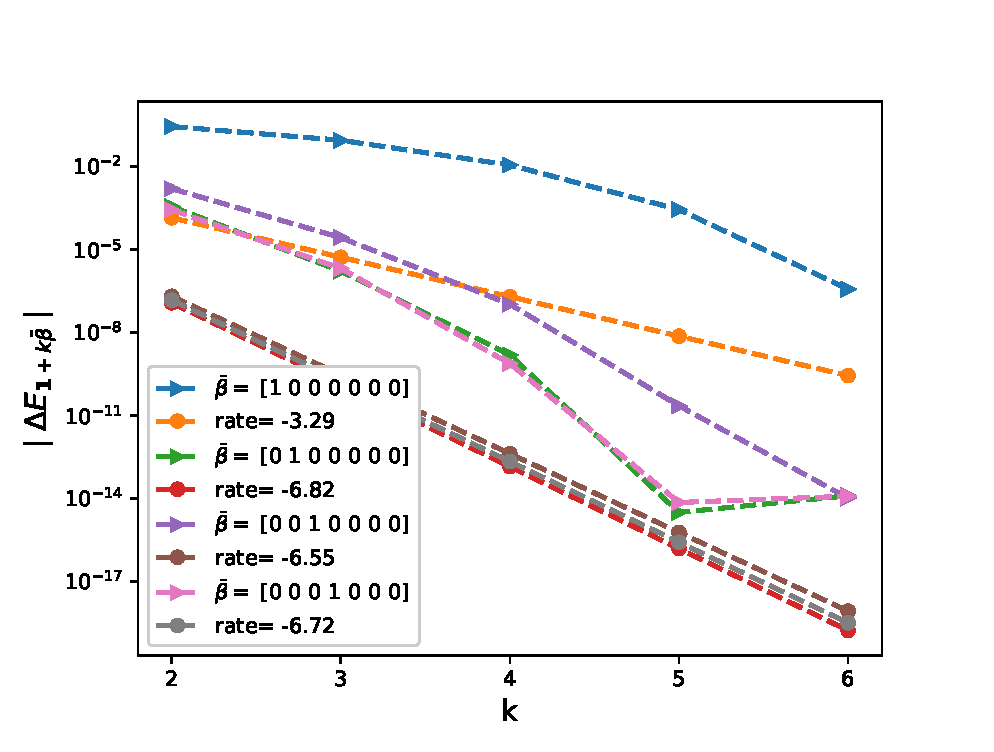
\includegraphics[width=\linewidth]{./figures/Heston_single_call_ABR_moment_matching/mixed_rates/set2/N_4/first_difference_heston_4steps_hierarchical}
		\caption{}
		\label{fig:2}
	\end{subfigure}\hfil %% <-- added
	\begin{subfigure}{0.4\textwidth}
		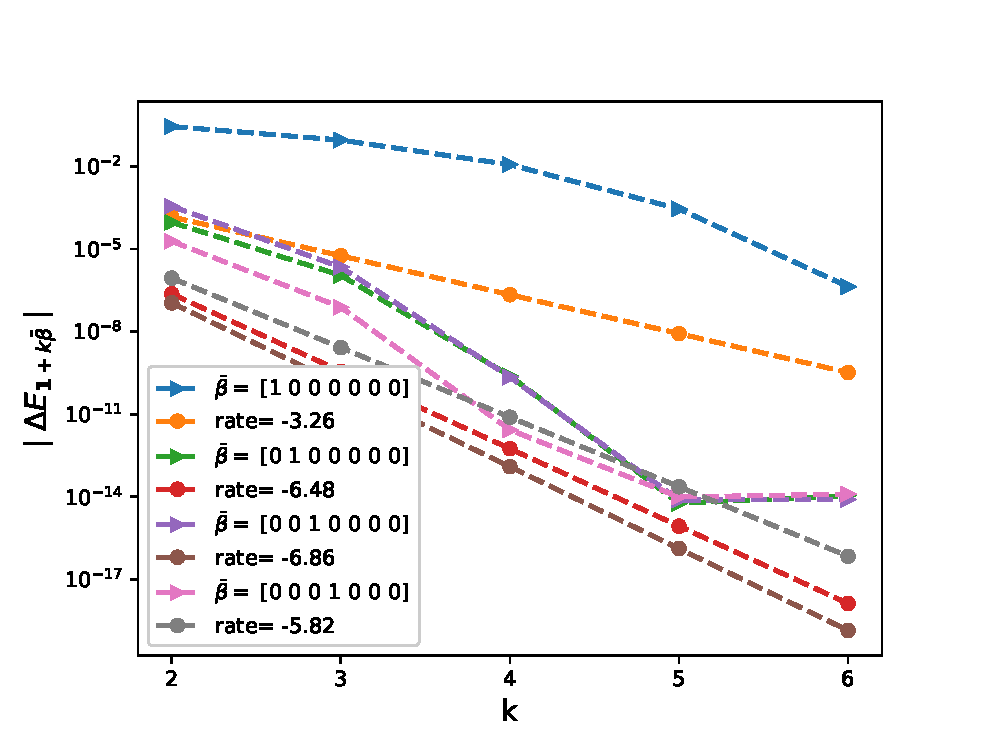
\includegraphics[width=\linewidth]{./figures/Heston_single_call_QE_moment_matching/mixed_rates/set2/N_4/first_difference_heston_4steps_hierarchical}
		\caption{}
		\label{fig:3}
	\end{subfigure}
		\begin{subfigure}{0.4\textwidth}
		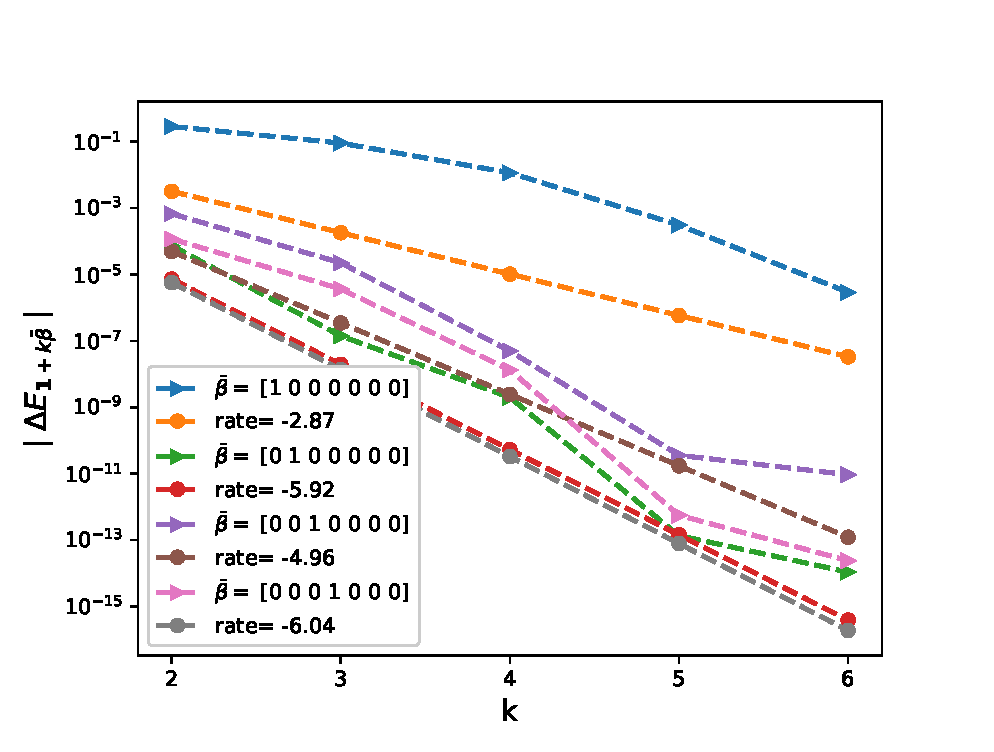
\includegraphics[width=\linewidth]{./figures/Heston_single_call_smooth_vol/mixed_rates/set2/N_4/first_difference_heston_4steps_spot_hierarchical_2}
		\caption{}
		\label{fig:4}
	\end{subfigure}
	\caption{The rate of error convergence of first order differences $\abs{\Delta \text{E}_{\boldsymbol{\beta}}}$, defined by \eqref{eq:Work_error_contributions}, ($\boldsymbol{\beta}=\mathbf{1}+k \bar{\boldsymbol{\beta}}$) for the example of single call option under Heston model, with parameters given by Set $1$ in Table \ref{table:Reference solution, for different parameter constellations.},  using $N=4$ time steps. In this case, we just show  the first  $4$ dimensions which are used for the volatility noise (mainly $dW_v$ in \eqref{eq:dynamics Heston}). (a) using full truncation as in Section \ref{sec:Discretization of Heston model with a non smooth transformations for the volatility process}, (b) using the ABR scheme as in Section \ref{sec:The ABR method}, (c) using the QE scheme as in Section \ref{sec:The QE method}, (d) using the smooth transformation as in Section \ref{sec:Discretization of Heston model with the volatility process Simulated using the sum of  Ornstein-Uhlenbeck (Bessel) processes}.}
	\label{fig:first_diff_Heston_call_N_4_set2}	
\end{figure}
\FloatBarrier


\subsubsection*{Mixed differences for the case of Set 2 parameters}

\FloatBarrier
\begin{figure}[htb]
	\centering % <-- added
	\begin{subfigure}{0.4\textwidth}
		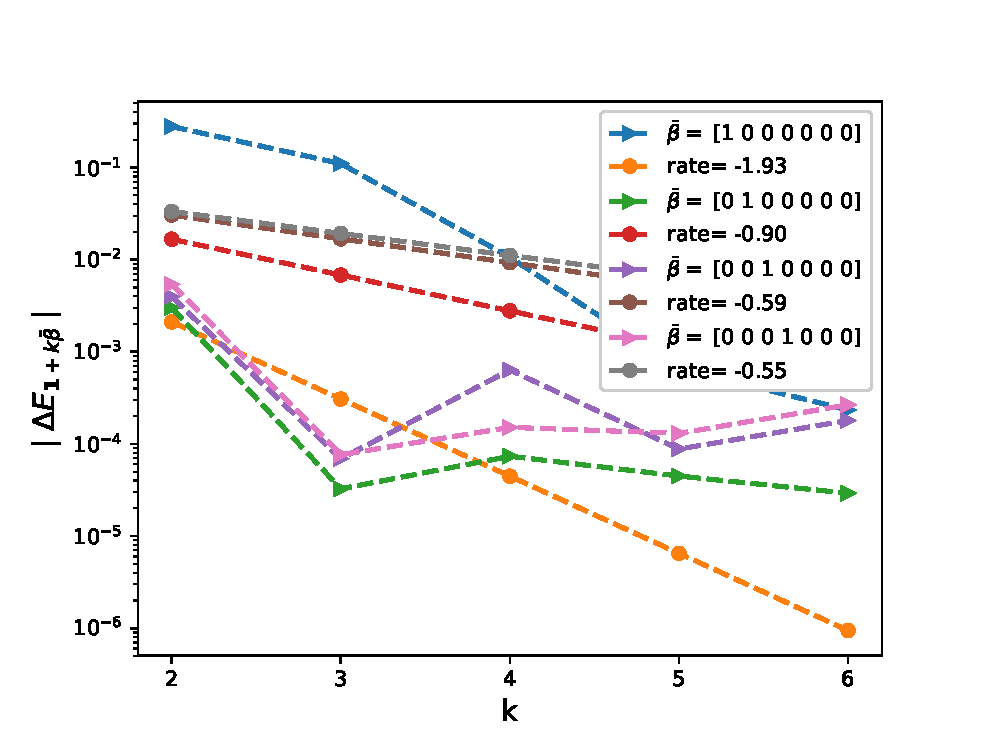
\includegraphics[width=\linewidth]{./figures/Heston_single_call_full_truncation_vol/mixed_rates/set3/N_4/first_difference_heston_4steps_hierarchical}
		\caption{}
		\label{fig:1}
	\end{subfigure}\hfil % <-- added
	\begin{subfigure}{0.4\textwidth}
		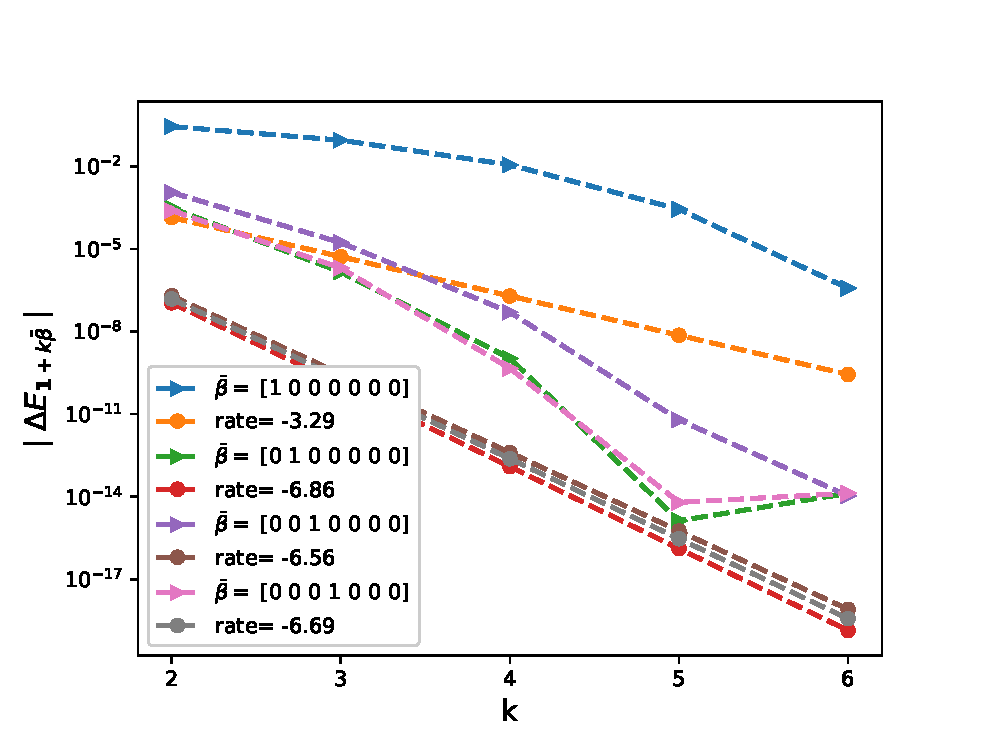
\includegraphics[width=\linewidth]{./figures/Heston_single_call_ABR_moment_matching/mixed_rates/set3/N_4/first_difference_heston_4steps_hierarchical}
		\caption{}
		\label{fig:2}
	\end{subfigure}\hfil % <-- added
	\begin{subfigure}{0.4\textwidth}
		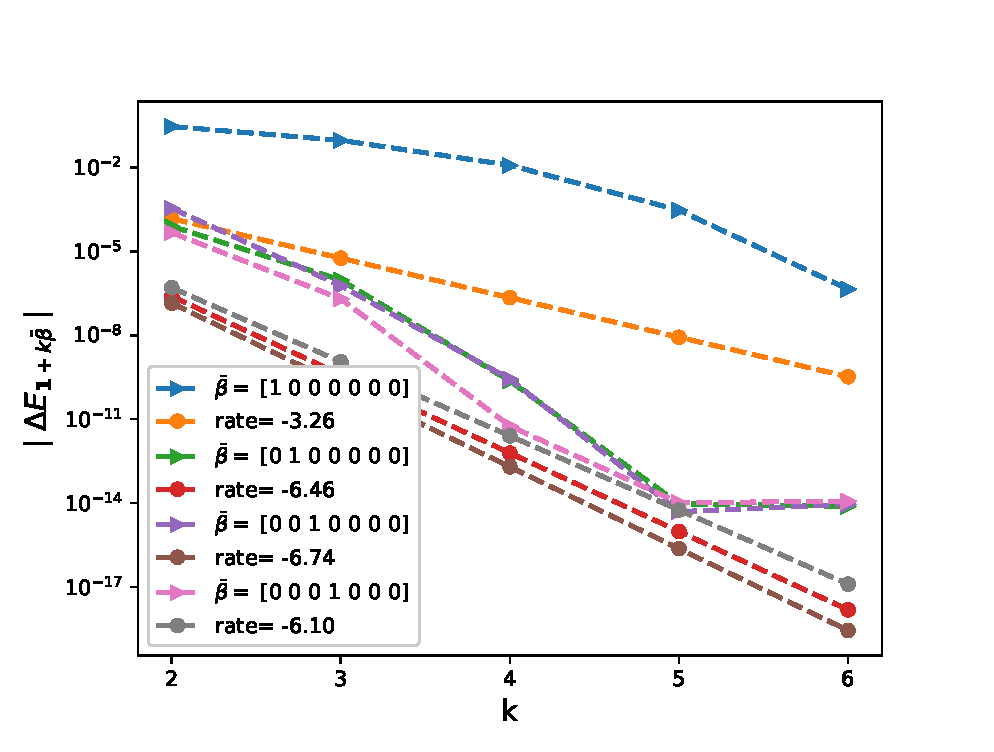
\includegraphics[width=\linewidth]{./figures/Heston_single_call_QE_moment_matching/mixed_rates/set3/N_4/first_difference_heston_4steps_hierarchical}
		\caption{}
		\label{fig:3}
	\end{subfigure}
		\begin{subfigure}{0.4\textwidth}
		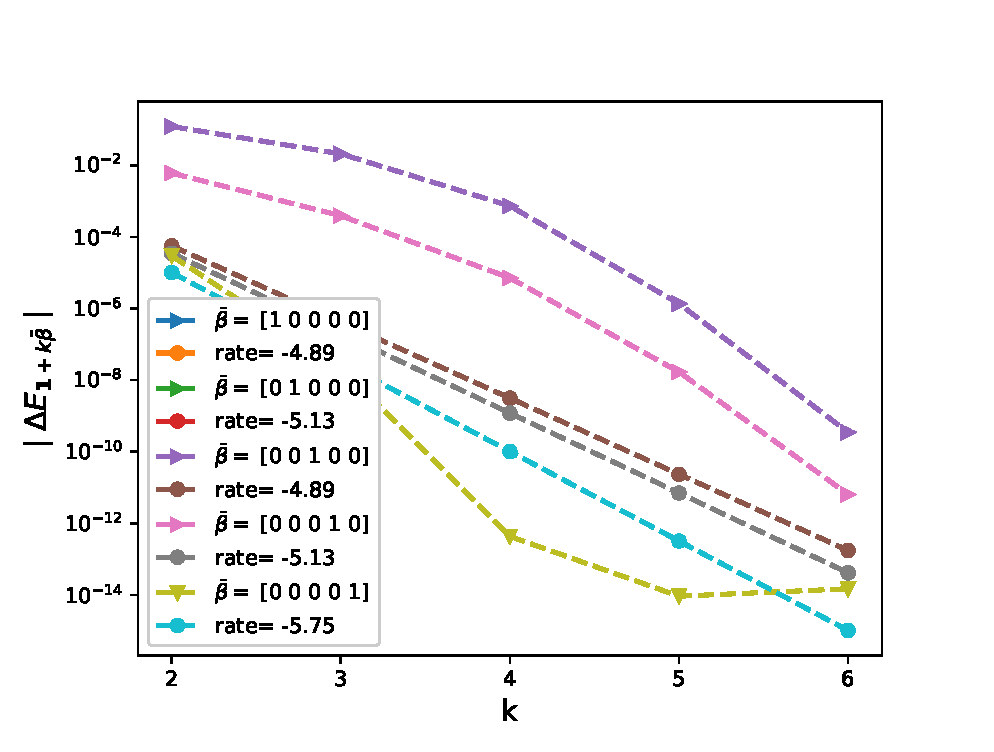
\includegraphics[width=\linewidth]{./figures/Heston_single_call_smooth_vol/mixed_rates/set3/N_2/first_difference_heston_2steps_spot_hierarchical}
		\caption{}
		\label{fig:4}
	\end{subfigure}
	\caption{The rate of error convergence of first order differences $\abs{\Delta \text{E}_{\boldsymbol{\beta}}}$, defined by \eqref{eq:Work_error_contributions}, ($\boldsymbol{\beta}=\mathbf{1}+k \bar{\boldsymbol{\beta}}$) for the example of single call option under Heston model, with parameters given by Set $2$ in Table \ref{table:Reference solution, for different parameter constellations.}, using $N=4$ time steps. In this case, we just show  the first  $4$ dimensions which are used for the volatility noise (mainly $dW_v$ in \eqref{eq:dynamics Heston}). (a) using full truncation as in Section \ref{sec:Discretization of Heston model with a non smooth transformations for the volatility process}, (b) using the ABR scheme as in Section \ref{sec:The ABR method}, (c) using the QE scheme as in Section \ref{sec:The QE method}, (d) using the smooth transformation as in Section \ref{sec:Discretization of Heston model with the volatility process Simulated using the sum of  Ornstein-Uhlenbeck (Bessel) processes}, here $N=2$.}
	\label{fig:first_diff_Heston_call_N_4_set3}	
\end{figure}
\FloatBarrier
\subsubsection*{Mixed differences for the case of Set 3 parameters}

\FloatBarrier
\begin{figure}[htb]
	\centering % <-- added
	\begin{subfigure}{0.4\textwidth}
		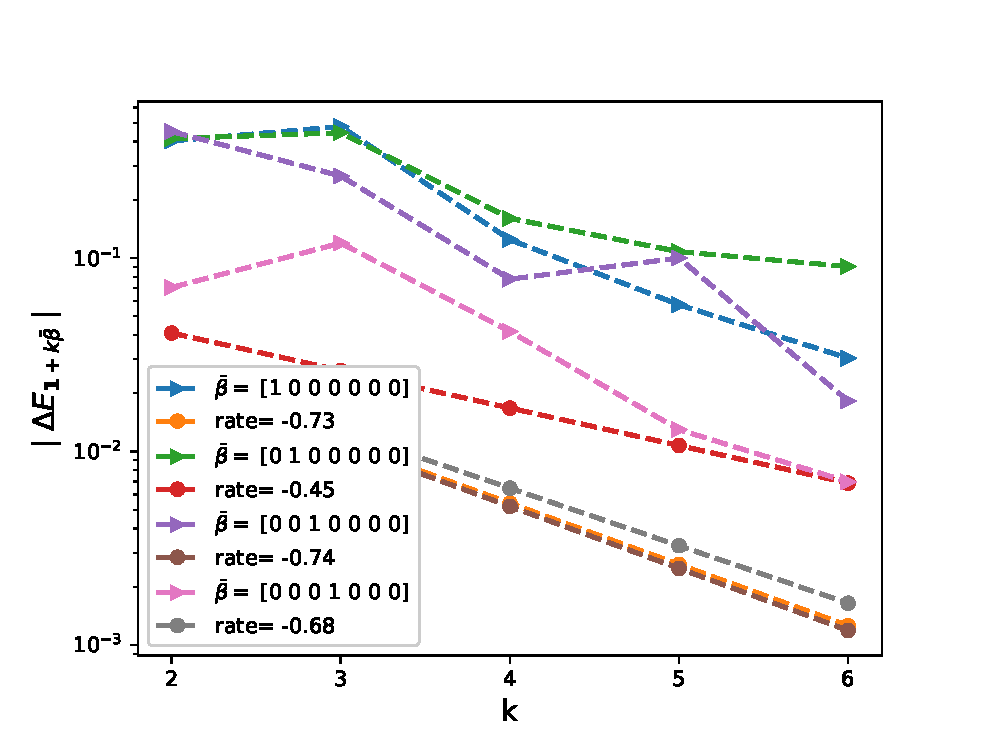
\includegraphics[width=\linewidth]{./figures/Heston_single_call_full_truncation_vol/mixed_rates/set4/N_4/first_difference_heston_4steps_hierarchical}
		\caption{}
		\label{fig:1}
	\end{subfigure}\hfil % <-- added
	\begin{subfigure}{0.4\textwidth}
		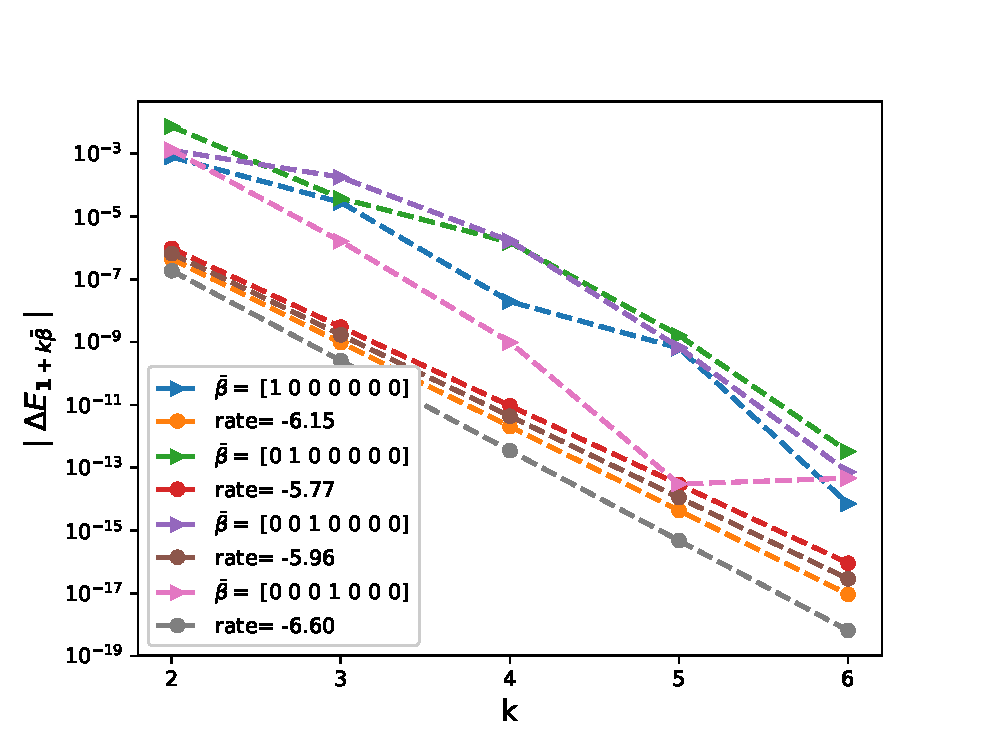
\includegraphics[width=\linewidth]{./figures/Heston_single_call_ABR_moment_matching/mixed_rates/set4/N_4/first_difference_heston_4steps_hierarchical}
		\caption{}
		\label{fig:2}
	\end{subfigure}\hfil % <-- added
	\begin{subfigure}{0.4\textwidth}
		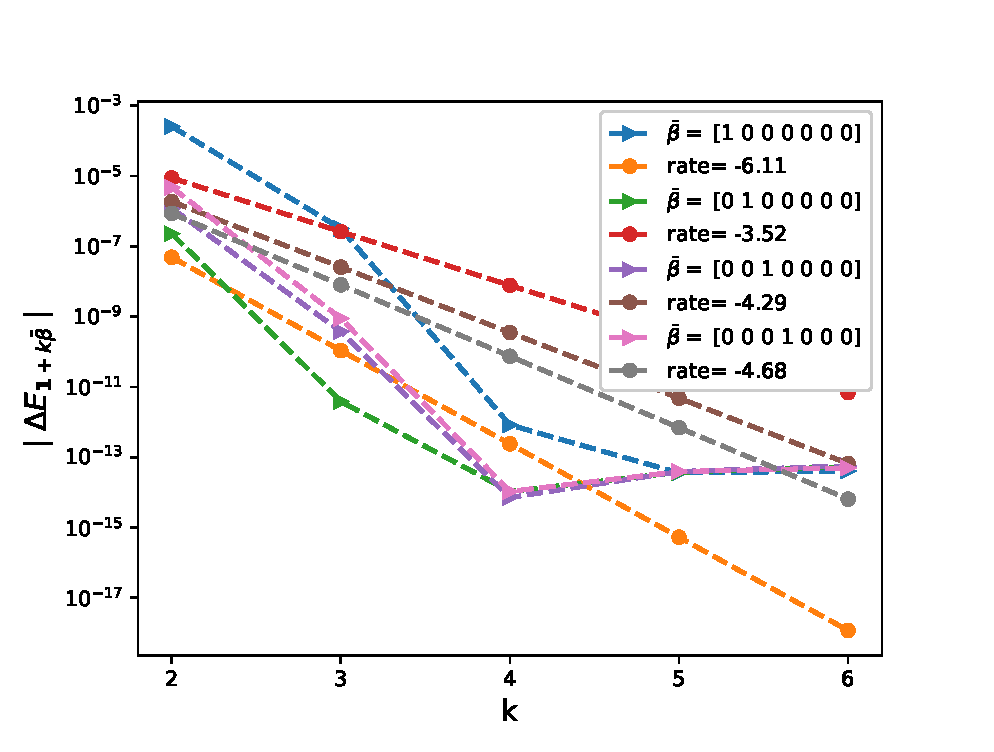
\includegraphics[width=\linewidth]{./figures/Heston_single_call_QE_moment_matching/mixed_rates/set4/N_4/first_difference_heston_4steps_hierarchical}
		\caption{}
		\label{fig:3}
	\end{subfigure}
		\begin{subfigure}{0.4\textwidth}
		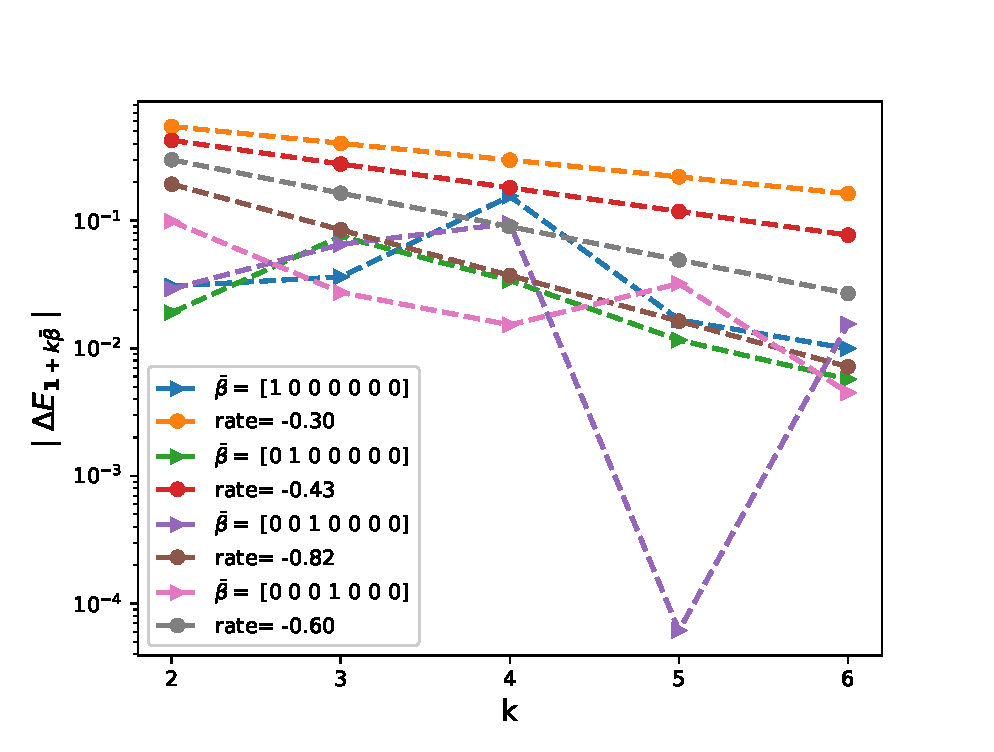
\includegraphics[width=\linewidth]{./figures/Heston_single_call_smooth_vol/mixed_rates/set4/N_4/first_difference_heston_4steps_spot_hierarchical}
		\caption{}
		\label{fig:4}
	\end{subfigure}
	\caption{The rate of error convergence of first order differences $\abs{\Delta \text{E}_{\boldsymbol{\beta}}}$, defined by \eqref{eq:Work_error_contributions}, ($\boldsymbol{\beta}=\mathbf{1}+k \bar{\boldsymbol{\beta}}$) for the example of single call option under Heston model, with parameters given by Set $3$ in Table \ref{table:Reference solution, for different parameter constellations.}, using $N=4$ time steps. In this case, we just show  the first  $4$ dimensions which are used for the volatility noise (mainly $dW_v$ in \eqref{eq:dynamics Heston}). (a) using full truncation as in Section \ref{sec:Discretization of Heston model with a non smooth transformations for the volatility process}, (b) using the ABR scheme as in Section \ref{sec:The ABR method}, (c) using the QE scheme as in Section \ref{sec:The QE method}, (d) using the smooth transformation as in Section \ref{sec:Discretization of Heston model with the volatility process Simulated using the sum of  Ornstein-Uhlenbeck (Bessel) processes}.}
	\label{fig:first_diff_Heston_call_N_4_set4}	
\end{figure}
\FloatBarrier
  
\subsubsection*{Mixed differences for the case of Set 4 parameters}

\FloatBarrier
\begin{figure}[htb]
	\centering % <-- added
	\begin{subfigure}{0.4\textwidth}
		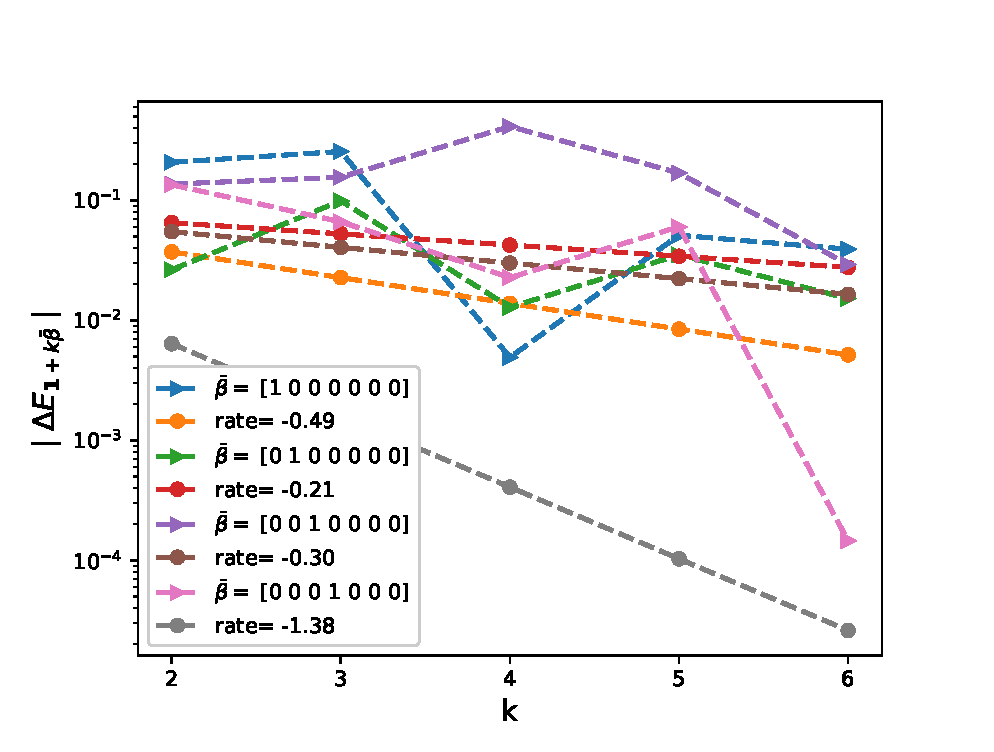
\includegraphics[width=\linewidth]{./figures/Heston_single_call_full_truncation_vol/mixed_rates/set5/N_4/first_difference_heston_4steps_hierarchical}
		\caption{}
		\label{fig:1}
	\end{subfigure}\hfil % <-- added
	\begin{subfigure}{0.4\textwidth}
		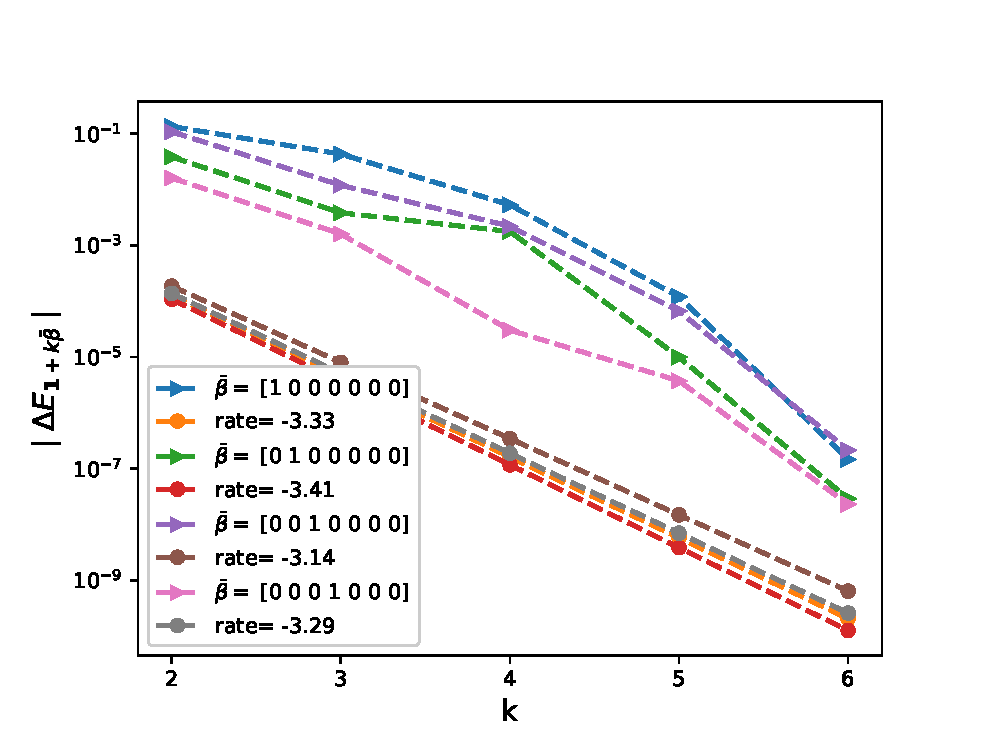
\includegraphics[width=\linewidth]{./figures/Heston_single_call_ABR_moment_matching/mixed_rates/set5/N_4/first_difference_heston_4steps_hierarchical}
		\caption{}
		\label{fig:2}
	\end{subfigure}\hfil % <-- added
		\begin{subfigure}{0.4\textwidth}
		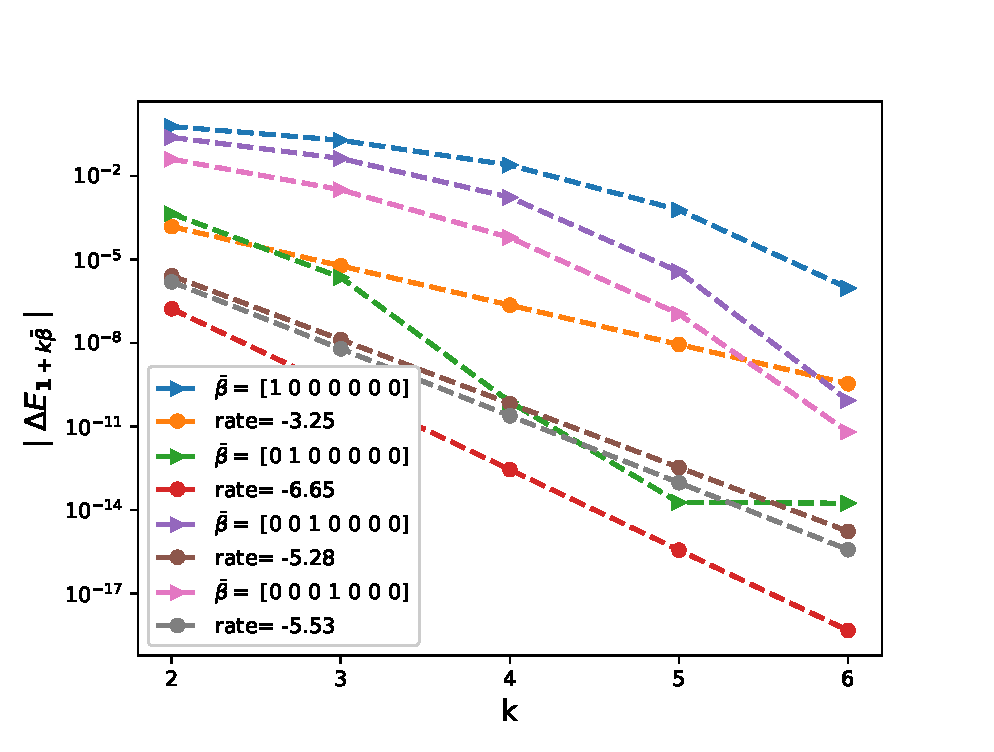
\includegraphics[width=\linewidth]{./figures/Heston_single_call_QE_moment_matching/mixed_rates/set5/N_4/first_difference_heston_4steps_hierarchical}
		\caption{}
		\label{fig:3}
	\end{subfigure}
	\caption{The rate of error convergence of first order differences $\abs{\Delta \text{E}_{\boldsymbol{\beta}}}$, defined by \eqref{eq:Work_error_contributions}, ($\boldsymbol{\beta}=\mathbf{1}+k \bar{\boldsymbol{\beta}}$) for the example of single call option under Heston model, with parameters given by Set $4$ in Table \ref{table:Reference solution, for different parameter constellations.}, using $N=4$ time steps. In this case, we just show  the first  $4$ dimensions which are used for the volatility noise (mainly $dW_v$ in \eqref{eq:dynamics Heston}).(a) using full truncation as in Section \ref{sec:Discretization of Heston model with a non smooth transformations for the volatility process}, (b) using the ABR scheme as in Section \ref{sec:The ABR method}, (c) using the QE scheme as in Section \ref{sec:The QE method}.}
	\label{fig:first_diff_Heston_call_N_4_set5}	
\end{figure}
\FloatBarrier

\subsubsection{Comparison in terms of  the weak error behavior (under process)}
 %%%%%%%%%%%%%%%%%%%%%%%%%%%%%%%%%%%%%%%%%%
%References
%%%%%%%%%%%%%%%%%%%%%%%%%%%%%%%%%%%%%%%%%%

\bibliographystyle{plain}
\bibliography{smoothing} 


%\appendix
%\section{Numerical comparison between MISC and MC}
\subsection{Case of set $1$ parameters in table \ref{table:Reference solution, using MC with $500$ time steps, of Call option price under rBergomi model, for different parameter constellation.}}\label{appendix:Case of set 1 parameters}


\begin{table}[h!]
	\centering
	\begin{tabular}{l*{6}{c}r}
		Method \textbackslash  Steps            & $2$ & $4$ & $8$ & $16$  \\
		\hline
%		MISC ($TOL_{\text{MISC}}=5.10^{-1}$)  & $\underset{0.0062}{\mathbf{  0.0868}}$ & $\underset{ 0.0040}{\mathbf{0.0563}}$ & $\underset{ 0.0040}{\mathbf{0.0563}}$ & $\underset{0.0014}{\mathbf{0.0197}}$  \\
		MISC ($TOL_{\text{MISC}}=10^{-1}$)  & $\underset{0.0062}{\mathbf{  0.0868}}$ & $\underset{ 0.0040}{\mathbf{0.0563}}$& $\underset{0.0049}{\mathbf{0.0681}}$ & $\underset{0.0035
		}{\mathbf{0.0492}}$  \\
%		MISC ($TOL_{\text{MISC}}=5.10^{-2}$)  &$\underset{0.0062}{\mathbf{  0.0868}}$ & $\underset{0.0042}{\mathbf{0.0591}}$ & $\underset{0.0021}{\mathbf{0.0288
%		}}$ & $\underset{0.0057}{\mathbf{0.0800}}$  \\
		MISC ($TOL_{\text{MISC}}=10^{-2}$)  & $\underset{ 0.0001
		}{\mathbf{\red{  0.0017}}}$ & $\underset{ 0.0023}{\mathbf{ 0.0324}}$ & $\underset{0.0016
		}{\mathbf{0.0218
		}}$ & $\underset{0.0005}{\mathbf{\red{0.0070}}}$  \\
		MISC ($TOL_{\text{MISC}}=10^{-3}$)  & $\underset{ 0.0001
		}{\mathbf{  0.0017}}$ & $\underset{1.0e-05
		}{\mathbf{ \red{1.4e-04
		}}}$ & $\underset{3.5e-04
		}{\mathbf{  0.0049
		}}$ & $\underset{0.0005}{\mathbf{ 0.0070}}$  \\
%		MISC ($TOL_{\text{MISC}}=5.10^{-4}$)  & $\underset{ 0.0001
%		}{\mathbf{  0.0017}}$ & $\underset{1.0e-05
%		}{\mathbf{ 1.4e-04
%		}}$ & $\underset{1.5e-04
%		}{\mathbf{    0.0021
%		}}$ & $\underset{-}{\mathbf{-}}$  \\
		MISC ($TOL_{\text{MISC}}=10^{-4}$)  & $\underset{ 0.0001
		}{\mathbf{  0.0017}}$ & $\underset{1.0e-05
		}{\mathbf{ 1.4e-04
		}}$ & $\underset{(  4.9e-05)
		}{\mathbf{\red{6.9e-04}
		}}$ & $\underset{-}{\mathbf{-}}$  \\
		\hline
	\end{tabular}
	\caption{Quadrature error of MISC,  with different tolerances, to compute call option price for different number of time steps. Case  set $1$ parameters in table \ref{table:Reference solution, using MC with $500$ time steps, of Call option price under rBergomi model, for different parameter constellation.}, without Richardson extrapolation. The numbers between parentheses are the corresponding absolute errors. The values marked in red correspond to stable quadrature errors for MISC, and will be used for complexity comparison against MC.}
	\label{Quadrature error of MISC to compute Call option price of the different tolerances for different number of time steps. Case  set $1$ parameters, without Richardson extrapolation. The numbers between parentheses are the corresponding absolute errors.}
\end{table}



\begin{table}[!h]
	\centering
	\begin{tabular}{l*{6}{c}r}
		Method \textbackslash  Steps            & $1-2$ & $2-4$ & $4-8$  \\
		\hline
%		MISC ($TOL_{\text{MISC}}=5.10^{-1}$)  & $\underset{(  0.0120)}{\mathbf{   0.1685}}$ & $\underset{(0.0031)}{\mathbf{0.0435}}$ & $\underset{(0.0014
%			)}{\mathbf{ 0.0197}}$  \\
		MISC ($TOL_{\text{MISC}}=10^{-1}$)  & $\underset{(  0.0120)}{\mathbf{   0.1685}}$ & $\underset{(0.0031)}{\mathbf{0.0435}}$ & $\underset{(0.0064)}{\mathbf{0.0899}}$  \\
%		MISC ($TOL_{\text{MISC}}=5.10^{-2}$)  & $\underset{(  0.0120)}{\mathbf{   0.1685}}$ & $\underset{(0.0079)}{\mathbf{0.1109}}$ & $\underset{(0.0052)}{\mathbf{0.0730}}$   \\
		MISC ($TOL_{\text{MISC}}=10^{-2}$)  & $\underset{(7e-07)}{\mathbf{1e-05}}$ &    $\underset{(0.0029)}{\mathbf{0.0407}}$ & $\underset{(0.0024  )}{\mathbf{0.0337}}$  \\
		MISC ($TOL_{\text{MISC}}=10^{-3}$)  & $\underset{(0.0013)}{\mathbf{
				\red{0.0183}}}$ &    $\underset{(0.0014
			)}{\mathbf{\red{0.0197}}}$ & $\underset{(0.0001)}{\mathbf{ \red{0.0014}
		}}$   \\
		
%		MISC ($TOL_{\text{MISC}}=10^{-4}$)  & $\underset{(0.0013)}{\mathbf{
%				0.0183}}$ &    $\underset{(0.0011
%			
%			)}{\mathbf{0.0154}}$   \\
		\hline
	\end{tabular}
	\caption{Quadrature error of MISC, with different tolerances,  to compute call option price  for different number of time steps. Case set $1$ parameters in table \ref{table:Reference solution, using MC with $500$ time steps, of Call option price under rBergomi model, for different parameter constellation.}, with Richardson extrapolation(level $1$). The numbers between parentheses are the corresponding absolute errors. The values marked in red correspond to stable quadrature errors for MISC, and will be used for complexity comparison against MC.}
	\label{Quadrature error of MISC to compute Call option price of the different tolerances for different number of time steps. Case set $1$ parameters, with Richardson extrapolation(level $1$). The numbers between parentheses are the corresponding absolute errors.}
\end{table}





\begin{table}[!h]
	\centering
	\begin{tabular}{l*{6}{c}r}
		Method \textbackslash  Steps            & $1-2-4$ & $2-4-8$  \\
		\hline
%		MISC ($TOL_{\text{MISC}}=5.10^{-1}$)  & $\underset{(     0.0017)}{\mathbf{    0.0239}}$ & $\underset{(0.0009)}{\mathbf{0.0126}}$ \\
		MISC ($TOL_{\text{MISC}}=10^{-1}$)  & $\underset{(   0.0041)}{\mathbf{  0.0576}}$ & $\underset{(0.0037)}{\mathbf{0.0520}}$  \\
%		MISC ($TOl=5.10^{-2}$)  & $\underset{(  0.0125)}{\mathbf{   0.1755}}$ & $\underset{(0.0072)}{\mathbf{0.1011}}$   \\
		MISC ($TOL_{\text{MISC}}=10^{-2}$)  & $\underset{(0.0031)}{\mathbf{0.0435}}$ &    $\underset{(0.0019)}{\mathbf{0.0267}}$   \\
		
		MISC ($TOL_{\text{MISC}}=5.10^{-3}$)  & $\underset{(0.0012)}{\mathbf{
				\red{0.0169}}}$ &    $\underset{(0.0002
			)}{\mathbf{\red{ 0.0028}}}$ \\
%		MISC ($TOL_{\text{MISC}}=10^{-3}$)  & $\underset{(1.0e-05
%			)}{\mathbf{
%				1.4e-04}}$ &    $\underset{(0.0002
%			)}{\mathbf{ 0.0028}}$ \\
%		
%		MISC ($TOL_{\text{MISC}}=10^{-4}$)  & $\underset{(1.0e-05
%			)}{\mathbf{
%				1.4e-04}}$&    $\underset{(-
%			
%			)}{\mathbf{-}}$   \\
		\hline
	\end{tabular}
	\caption{Quadrature error of MISC, with different tolerances, to compute call option price for different number of time steps. Case set $1$ parameters in table \ref{table:Reference solution, using MC with $500$ time steps, of Call option price under rBergomi model, for different parameter constellation.}, with Richardson extrapolation(level $2$). The numbers between parentheses are the corresponding absolute errors. The values marked in red correspond to stable quadrature errors for MISC, and will be used for complexity comparison against MC.}
	\label{Quadrature error of MISC to compute Call option price of the different tolerances for different number of time steps. Case set $1$ parameters, with Richardson extrapolation(level $2$). The numbers between parentheses are the corresponding absolute errors.}
\end{table}


\FloatBarrier


\subsection{Case of set $2$ parameters in table \ref{table:Reference solution, using MC with $500$ time steps, of Call option price under rBergomi model, for different parameter constellation.} }
\label{appendix:Case of set $2$ parameters_linear}



\begin{table}[h!]
	\centering
	\begin{tabular}{l*{6}{c}r}
		Method \textbackslash  Steps            & $2$ & $4$ & $8$ \\
		\hline
%		MISC ($TOL_{\text{MISC}}=5.10^{-1}$)  & $\underset{(     0.0121)}{\mathbf{
%				0.1525}}$ & $\underset{(    0.0097)}{\mathbf{      0.1231
%		}}$ & $\underset{(   0.0107)}{\mathbf{0.1353
%		}}$ \\
		MISC ($TOL_{\text{MISC}}=10^{-1}$)  & $\underset{(     0.0121)}{\mathbf{
				0.1525}}$ & $\underset{(    0.0097)}{\mathbf{      0.1231
		}}$ & $\underset{( 0.0123
			
			)}{\mathbf{    0.1555}}$   \\
%		MISC ($TOL_{\text{MISC}}=5.10^{-2}$)  &$\underset{(     0.0121)}{\mathbf{
%				0.1525}}$& $\underset{(     0.0134
%			)}{\mathbf{  
%				0.1686}}$ & $\underset{(   0.0065)}{\mathbf{ 0.0823}}$  \\
		MISC ($TOL_{\text{MISC}}=10^{-2}$)  & $\underset{(    0.0099
			)}{\mathbf{     0.1247
		}}$ & $\underset{(   5.0e-05)}{\mathbf{\red{  6.3e-04}
		}}$ & $\underset{(0.0004)}{\mathbf{\red{0.0053}}}$  \\
		MISC ($TOL_{\text{MISC}}=10^{-3}$)        & $\underset{(    
			0.0023)}{\mathbf{0.0288}}$  &$\underset{(   5.0e-05)}{\mathbf{  6.3e-04
		}}$ & $\underset{(0.0004)}{\mathbf{0.0053}}$  \\
		MISC ($TOL_{\text{MISC}}=10^{-4}$)        & $\underset{(2.0e-05)}{\mathbf{  \red{ 2.5e-04}}} $ &$\underset{(   5.0e-05)}{\mathbf{ 6.3e-04
		}}$ &  $-$ \\	
		
		\hline
	\end{tabular}
	\caption{Quadrature error of MISC, with different tolerances, to compute call option price  for different number of time steps. Case  set $2$ parameters in table \ref{table:Reference solution, using MC with $500$ time steps, of Call option price under rBergomi model, for different parameter constellation.}, without Richardson extrapolation. The numbers between parentheses are the corresponding absolute errors. The values marked in red correspond to stable quadrature errors for MISC, and will be used for complexity comparison against MC.}
	\label{Quadrature error of MISC to compute Call option price of the different tolerances for different number of time steps. Case  set $2$ parameters, without Richardson extrapolation. The numbers between parentheses are the corresponding absolute errors,linear}
\end{table}


\begin{table}[h!]
	\centering
	\begin{tabular}{l*{6}{c}r}
		Method \textbackslash  Steps            & $1-2$ & $2-4$ & $4-8$ \\
		\hline
%		MISC ($TOL_{\text{MISC}}=5.10^{-1}$)  & $\underset{ 0.0292}{\mathbf{
%				0.3687}}$ & $\underset{ 0.0090}{\mathbf{    0.1136}}$ & $\underset{    0.0117
%		}{\mathbf{
%				0.1477
%		}}$ \\
		MISC ($TOL_{\text{MISC}}=10^{-1}$)  & $\underset{ 0.0292}{\mathbf{
				0.3687}}$ & $\underset{ 0.0090}{\mathbf{    0.1136}}$ & $\underset{  0.0102}{\mathbf{  0.1288
		}}$   \\
		MISC ($TOL_{\text{MISC}}=5.10^{-2}$)  & $\underset{ 0.0292}{\mathbf{
				0.3687}}$& $\underset{  0.0130}{\mathbf{
				0.1641
		}}$ & $\underset{0.0008}{\mathbf{\red{0.0101}}}$  \\
		MISC ($TOL_{\text{MISC}}=10^{-2}$)  & $\underset{   0.0096
		}{\mathbf{    0.1212
		}}$ & $\underset{0.0008}{\mathbf{
				\red{0.0101}}}$ & $\underset{0.0008 }{\mathbf{
				0.0101}}$  \\
		MISC ($TOL_{\text{MISC}}=10^{-3}$)  & $\underset{     0.0055
		}{\mathbf{ \red{    0.0694}
		}}$ & $\underset{0.0008}{\mathbf{
				0.0101}}$ & $\underset{-}{\mathbf{-}}$   \\
		
%		MISC ($TOL_{\text{MISC}}=10^{-4}$)  & $\underset{  0.0051}{\mathbf{    0.0644		}}$ & $\underset{-}{\mathbf{-}}$ & $\underset{-}{\mathbf{-}}$   \\
%		
		\hline
	\end{tabular}
	\caption{Quadrature error of MISC, with different tolerances,   to compute call option price for different number of time steps. Case set $2$ parameters in table \ref{table:Reference solution, using MC with $500$ time steps, of Call option price under rBergomi model, for different parameter constellation.}, with Richardson extrapolation(level $1$). The numbers between parentheses are the corresponding absolute errors. The values marked in red correspond to stable quadrature errors for MISC, and will be used for complexity comparison against MC.}
	\label{Quadrature error of MISC to compute Call option price of the different tolerances for different number of time steps. Case set $2$ parameters, with Richardson extrapolation(level $1$). The numbers between parentheses are the corresponding absolute errors,linear}
\end{table}



\begin{table}[!h]
	\centering
	\begin{tabular}{l*{6}{c}r}
		Method \textbackslash  Steps            & $1-2-4$ & $2-4-8$  \\
		\hline
%		MISC ($TOL_{\text{MISC}}=5.10^{-1}$)  & $\underset{(    0.0014)}{\mathbf{  0.0177}}$ & $\underset{(0.0123)}{\mathbf{0.1553}}$ \\
		MISC ($TOL_{\text{MISC}}=10^{-1}$)  & $\underset{(    0.0014)}{\mathbf{  0.0177}}$ & $\underset{(  0.0085)}{\mathbf{0.1073}}$  \\
		MISC ($TOL_{\text{MISC}}=5.10^{-2}$)  & $\underset{(  0.0200)}{\mathbf{  0.2525}}$ & $\underset{(0.0004)}{\mathbf{\red{0.0038}}}$   \\
		MISC ($TOL_{\text{MISC}}=10^{-2}$)  & $\underset{(0.0022)}{\mathbf{\red{0.0278}}}$ &     $\underset{(0.0004)}{\mathbf{0.0038}}$  \\
		
%		MISC ($TOL_{\text{MISC}}=5.10^{-3}$)  & $\underset{(0.0022)}{\mathbf{0.0278}}$&    $\underset{(-
%			)}{\mathbf{-}}$ \\
%		MISC ($TOL_{\text{MISC}}=10^{-3}$)  & $\underset{(0.0007
%			)}{\mathbf{
%				0.0088}}$ &    $\underset{(-
%			)}{\mathbf{ -}}$ \\
%		
		
		\hline
	\end{tabular}
	\caption{Quadrature error of MISC, with different tolerances, to compute Call option price   for different number of time steps. Case set $2$ parameters in table \ref{table:Reference solution, using MC with $500$ time steps, of Call option price under rBergomi model, for different parameter constellation.}, with Richardson extrapolation(level $2$). The numbers between parentheses are the corresponding absolute errors. The values marked in red correspond to stable quadrature errors for MISC, and will be used for complexity comparison against MC.}
	\label{Quadrature error of MISC to compute Call option price of the different tolerances for different number of time steps. Case set $2$ parameters, with Richardson extrapolation(level $2$). The numbers between parentheses are the corresponding absolute errors,linear}
\end{table}



\FloatBarrier

\subsection{Case of set $3$ parameters in table \ref{table:Reference solution, using MC with $500$ time steps, of Call option price under rBergomi model, for different parameter constellation.}}\label{appendix:Case of set 3 parameters}


\begin{table}[h!]
	\centering
	\begin{tabular}{l*{6}{c}r}
		Method \textbackslash  Steps            & $2$ & $4$ & $8$ & $16$  \\
		\hline
%		MISC ($TOL_{\text{MISC}}=5.10^{-1}$)  & $\underset{(   0.0011)}{\mathbf{  0.0088}}$ & $\underset{(
%			0.0018)}{\mathbf{ 0.0144}}$ & $\underset{( 0.0022)}{\mathbf{0.0176}}$ & $\underset{(  0.0022)}{\mathbf{ 0.0176}}$  \\
		MISC ($TOL_{\text{MISC}}=10^{-1}$)  & $\underset{(   0.0011)}{\mathbf{  0.0088}}$ & $\underset{(
			0.0018)}{\mathbf{ 0.0144}}$& $\underset{( 0.0022)}{\mathbf{0.0176}}$  & $\underset{(  0.0020)}{\mathbf{ 0.0160}}$   \\
%		MISC ($TOL_{\text{MISC}}=5.10^{-2}$)  &$\underset{(   0.0011)}{\mathbf{  0.0088}}$ & $\underset{(
%			0.0018)}{\mathbf{ 0.0144}}$ & $\underset{( 0.0022)}{\mathbf{0.0176}}$  & $\underset{(0.0008)}{\mathbf{0.0064}}$  \\
		MISC ($TOL_{\text{MISC}}=10^{-2}$)  & $\underset{(   0.0011)}{\mathbf{  0.0088}}$ & $\underset{(0.0011
			)}{\mathbf{ 0.0088
		}}$ & $\underset{(0.0005)}{\mathbf{ 0.0040
		}}$ & $\underset{0.0001}{\mathbf{\red{0.0008}}}$  \\
		MISC ($TOL_{\text{MISC}}=10^{-3}$)  & $\underset{( 0.0002)}{\mathbf{    0.0016}}$ & $\underset{(0.0002
			)}{\mathbf{ 0.0016
		}}$ & $\underset{0.0001}{\mathbf{\red{0.0008}}}$ & $\underset{0.00005}{\mathbf{0.0004}}$ \\
		MISC ($TOL_{\text{MISC}}=10^{-4}$)  & $\underset{( 0.0001)}{\mathbf{    \red{0.0008}}}$ & $\underset{0.0001}{\mathbf{\red{0.0008}}}$& $\underset{0.0001}{\mathbf{0.0008}}$ & $\underset{-}{\mathbf{-}}$  \\
		
%		MISC ($TOL_{\text{MISC}}=10^{-5}$)  & $\underset{( 0.0001)}{\mathbf{    0.0008}}$ & $\underset{0.0001}{\mathbf{0.0008}}$& $\underset{0.0001}{\mathbf{0.0008}}$ & $\underset{-}{\mathbf{-}}$  \\
%		
		\hline
		
	\end{tabular}
	\caption{Quadrature error of MISC, with different tolerances,  to compute call option price  for different number of time steps. Case  set $3$ parameters in table \ref{table:Reference solution, using MC with $500$ time steps, of Call option price under rBergomi model, for different parameter constellation.}, without Richardson extrapolation. The numbers between parentheses are the corresponding absolute errors. The values marked in red correspond to stable quadrature errors for MISC, and will be used for complexity comparison against MC.}
	\label{Quadrature error of MISC to compute Call option price of the different tolerances for different number of time steps. Case  set $3$ parameters, without Richardson extrapolation. The numbers between parentheses are the corresponding absolute errors.}
\end{table}


\begin{table}[h!]
	\centering
	\begin{tabular}{l*{6}{c}r}
		Method \textbackslash  Steps            & $1-2$ & $2-4$ & $4-8$ & $8-16$  \\
		\hline
%		MISC ($TOL_{\text{MISC}}=5.10^{-1}$)  & $\underset{(0.0023)}{\mathbf{    0.0184
%		}}$  & $\underset{( 0.0031)}{\mathbf{ 0.0248}}$  & $\underset{(   0.0027)}{\mathbf{  0.0216}}$  & $\underset{(
%			0.0025
%			)}{\mathbf{  0.0200}}$  \\ 
		MISC ($TOL_{\text{MISC}}=10^{-1}$) & $\underset{(0.0023)}{\mathbf{    0.0184
		}}$  & $\underset{( 0.0031)}{\mathbf{ 0.0248}}$   & $\underset{(   0.0027)}{\mathbf{  0.0216}}$ & $\underset{(  0.0022)}{\mathbf{  0.0176}}$  \\ 
%		MISC ($TOL_{\text{MISC}}=5.10^{-2}$)  &  $\underset{(0.0023)}{\mathbf{    0.0184
%		}}$ & $\underset{( 0.0031)}{\mathbf{ 0.0248}}$   & $\underset{(   0.0027)}{\mathbf{  0.0216}}$  & $\underset{(  0.0008)}{\mathbf{  
%				0.0064}}$  \\ 
		MISC ($TOL_{\text{MISC}}=10^{-2}$)   & $\underset{(    0.0017
			)}{\mathbf{  0.0136}}$  & $\underset{(
			0.0021)}{\mathbf{   0.0168}}$  & $\underset{(0.0004)}{\mathbf{   0.0032
		}}$  & $\underset{(0.0001)}{\mathbf{\red{0.0008}}}$  \\ 
		MISC ($TOL_{\text{MISC}}=10^{-3}$)  & $\underset{(0.0001)}{\mathbf{\red{0.0008}}}$  & $\underset{(0.0006)}{\mathbf{  \red{0.0032}}}$   & $\underset{(0.0002)}{\mathbf{    \red{0.0016}}}$  &  $\underset{(0.0001)}{\mathbf{0.0008}}$  \\ 
		
%		MISC ($TOL_{\text{MISC}}=10^{-4}$)  & $\underset{(0.0001)}{\mathbf{0.0008}}$  & $\underset{(0.0006)}{\mathbf{ 0.0032}}$   & $\underset{(0.0002)}{\mathbf{   0.0016}}$ & $\underset{(-)}{\mathbf{-}}$  \\
%		
%		MISC ($TOL_{\text{MISC}}=10^{-5}$)    &  $\underset{(0.0001)}{\mathbf{0.0008}}$ & $\underset{(0.0006)}{\mathbf{  0.0032}}$   & $\underset{(0.0002)}{\mathbf{    0.0016}}$ & $\underset{(-)}{\mathbf{-}}$  \\
		
		\hline
	\end{tabular}
	\caption{Quadrature error of MISC, with different tolerances, to compute Call option price  for different number of time steps. Case set $3$ parameters in table \ref{table:Reference solution, using MC with $500$ time steps, of Call option price under rBergomi model, for different parameter constellation.}, with Richardson extrapolation(level $1$). The numbers between parentheses are the corresponding absolute errors. The values marked in red correspond to stable quadrature errors for MISC, and will be used for complexity comparison against MC.}
	\label{Quadrature error of MISC to compute Call option price of the different tolerances for different number of time steps. Case set $3$ parameters, with Richardson extrapolation(level $1$). The numbers between parentheses are the corresponding absolute errors.}
\end{table}




\FloatBarrier
\subsection{Case of set $4$ parameters in table \ref{table:Reference solution, using MC with $500$ time steps, of Call option price under rBergomi model, for different parameter constellation.}}\label{appendix:Case of set 4 parameters}



\begin{table}[h!]
	\centering
	\begin{tabular}{l*{6}{c}r}
		Method \textbackslash  Steps            & $2$ & $4$ & $8$ & $16$  \\
		\hline
%		MISC ($TOL_{\text{MISC}}=5.10^{-1}$)  & $\underset{(   0.0007)}{\mathbf{   0.0029}}$ & $\underset{(
%			
%			0.0013)}{\mathbf{     0.0054}}$ & $\underset{( 
%			0.0011)}{\mathbf{   0.0046}}$ & $\underset{(      0.0017)}{\mathbf{     0.0071
%		}}$  \\
		MISC ($TOL_{\text{MISC}}=10^{-1}$)  & $\underset{(   0.0007)}{\mathbf{   0.0029}}$ & $\underset{(
			
			0.0013)}{\mathbf{     0.0054}}$& $\underset{( 
			0.0011)}{\mathbf{   0.0046}}$  & $\underset{(    0.0016)}{\mathbf{     0.0066
		}}$   \\
%		MISC ($TOL_{\text{MISC}}=5.10^{-2}$)  &$\underset{(   0.0007)}{\mathbf{   0.0029}}$ & $\underset{(
%			
%			0.0013)}{\mathbf{     0.0054}}$ & $\underset{( 
%			0.0011)}{\mathbf{   0.0046}}$  & $\underset{(0.0008)}{\mathbf{
%				0.0033}}$  \\
		MISC ($TOL_{\text{MISC}}=10^{-2}$)  & $\underset{(   0.0007)}{\mathbf{   0.0029}}$ &$\underset{(
			
			0.0013)}{\mathbf{     0.0054}}$ & $\underset{(0.0005)}{\mathbf{    0.0021
		}}$ &  $\underset{2.0e-05}{\mathbf{\red{8.3e-05}}}$  \\
		MISC ($TOL_{\text{MISC}}=10^{-3}$)  & $\underset{(   0.0007)}{\mathbf{   0.0029}}$ & $\underset{(0.0005
			)}{\mathbf{ 
				0.0021
		}}$ & $\underset{3.0e-05}{\mathbf{\red{1.2e-04}}}$ &  $\underset{2.0e-05}{\mathbf{8.3e-05}}$  \\
		MISC ($TOL_{\text{MISC}}=10^{-4}$)  & $\underset{( 0.0001)}{\mathbf{    \red{0.0004}}}$ & $\underset{5.0e-05}{\mathbf{\red{2.1e-04}}}$& $\underset{3.0e-05}{\mathbf{1.2e-04}}$ & $\underset{-}{\mathbf{-}}$  \\
		
%		MISC ($TOL_{\text{MISC}}=10^{-5}$)  & $\underset{( 0.0001)}{\mathbf{   0.0004}}$ & $\underset{5.0e-05}{\mathbf{2.1e-04}}$& $\underset{3.0e-05}{\mathbf{1.2e-04}}$& $\underset{-}{\mathbf{-}}$  \\
		
		\hline
		
	\end{tabular}
	\caption{Quadrature error of MISC, with different tolerances,  to compute call option price for different number of time steps. Case  set $4$ parameters in table \ref{table:Reference solution, using MC with $500$ time steps, of Call option price under rBergomi model, for different parameter constellation.}, without Richardson extrapolation. The numbers between parentheses are the corresponding absolute errors. The values marked in red correspond to stable quadrature errors for MISC, and will be used for complexity comparison against MC.}
	\label{Quadrature error of MISC to compute Call option price of the different tolerances for different number of time steps. Case  set $4$ parameters, without Richardson extrapolation. The numbers between parentheses are the corresponding absolute errors.}
\end{table}



\FloatBarrier
\subsection{Case of set $5$ parameters in table \ref{table:Reference solution, using MC with $500$ time steps, of Call option price under rBergomi model, for different parameter constellation.}}\label{appendix:Case of set 5 parameters}


\begin{table}[h!]
	\centering
	\begin{tabular}{l*{6}{c}r}
		Method \textbackslash  Steps            & $2$ & $4$ & $8$ & $16$  \\
		\hline
%		MISC ($TOL_{\text{MISC}}=5.10^{-1}$)  & $\underset{(  0.0015
%			)}{\mathbf{     0.0264}}$ & $\underset{(    0.0023
%			)}{\mathbf{         0.0406}}$ & $\underset{(    0.0028)}{\mathbf{      0.0491
%		}}$ & $\underset{(      
%			0.0030)}{\mathbf{     0.0524
%		}}$  \\
		MISC ($TOL_{\text{MISC}}=10^{-1}$)  & $\underset{(  0.0015
			)}{\mathbf{     0.0264}}$& $\underset{(    0.0023
			)}{\mathbf{         0.0406}}$& $\underset{(    0.0028)}{\mathbf{      0.0491
		}}$  & $\underset{(      
			0.0030)}{\mathbf{     0.0524
		}}$   \\
%		MISC ($TOL_{\text{MISC}}=5.10^{-2}$)  &$\underset{(  0.0015
%			)}{\mathbf{     0.0264}}$ & $\underset{(    0.0023
%			)}{\mathbf{         0.0406}}$ & $\underset{(    0.0028)}{\mathbf{      0.0491
%		}}$ & $\underset{(  0.0019)}{\mathbf{
%				0.0331
%		}}$  \\
		MISC ($TOL_{\text{MISC}}=10^{-2}$)  & $\underset{(  0.0015
			)}{\mathbf{     0.0264}}$ &$\underset{(    0.0023
			)}{\mathbf{         0.0406}}$ & $\underset{(0.0005)}{\mathbf{    0.0021
		}}$ &  $\underset{0.0004}{\mathbf{    0.0065}}$  \\
		MISC ($TOL_{\text{MISC}}=10^{-3}$)  & $\underset{(      3.0e-05)}{\mathbf{    \red{5.3e-04}}}$ & $\underset{2.0e-05}{\mathbf{\red{3.5e-04}}}$& $\underset{1.9e-05}{\mathbf{\red{3.3e-04}}}$ &  $\underset{3.0e-05}{\mathbf{\red{5.3e-04}}}$  \\
%		MISC ($TOL_{\text{MISC}}=10^{-4}$)  & $\underset{(      3.0e-05)}{\mathbf{    5.3e-04}}$ & $\underset{2.0e-05}{\mathbf{3.5e-04}}$& $\underset{1.9e-05}{\mathbf{3.3e-04}}$ & $\underset{-}{\mathbf{-}}$  \\
%		
%		MISC ($TOL_{\text{MISC}}=10^{-5}$)  & $\underset{(      3.0e-05)}{\mathbf{    5.3e-04}}$ & $\underset{2.0e-05}{\mathbf{3.5e-04}}$& $\underset{1.9e-05}{\mathbf{3.3e-04}}$& $\underset{-}{\mathbf{-}}$  \\
%		
		\hline
		
	\end{tabular}
	\caption{Quadrature error of MISC, with  different tolerances,  to compute call option price  for different number of time steps. Case  set $5$ parameters in table \ref{table:Reference solution, using MC with $500$ time steps, of Call option price under rBergomi model, for different parameter constellation.}, without Richardson extrapolation. The numbers between parentheses are the corresponding absolute errors. The values marked in red correspond to stable quadrature errors for MISC, and will be used for complexity comparison against MC.}
	\label{Quadrature error of MISC to compute Call option price of the different tolerances for different number of time steps. Case  set $5$ parameters, without Richardson extrapolation. The numbers between parentheses are the corresponding absolute errors.}
\end{table}
\end{document}
%%% Local Variables:
%%% mode: latex
%%% TeX-master: t
%%% End:
